% !Mode:: "TeX:UTF-8"
% !TEX program  = xelatex
\documentclass[a4paper]{article}
\usepackage{amsmath}
\usepackage{amssymb}
\usepackage{ctex}
%\usepackage{braket}
\usepackage[european]{circuitikz}
\usepackage{multirow}
\usepackage{float}
\usepackage{geometry}
\geometry{left=2.5cm,right=2.5cm,bottom=2.5cm,top=2.5cm}
\title{模电实验报告3:负反馈放大电路实验}
\author{xy\quad 学号\quad 匡亚明学院}
\date{2019年2月29日}
\begin{document}
\maketitle
\bibliographystyle{unsrt}
%--------main-body------------

\section{实验目的}
\begin{enumerate}
\item 分析负反馈对放大器性能的影响。
\item 掌握测量负反馈放大器性能的测量方法。
\end{enumerate}

\section{实验仪器}
双踪示波器、信号发生器、交流毫伏表、数字万用表。

\section{预习内容}
\begin{enumerate}
\item 开环放大器和闭环放大器的放大倍数的计算方法。
\item 开环放大器和闭环放大器的输入、输出电阻的计算方法。
\item 负反馈闭环对放大器性能的影响。
\end{enumerate}
%--------figure 1-----------------
\begin{figure}[!h]
\centering
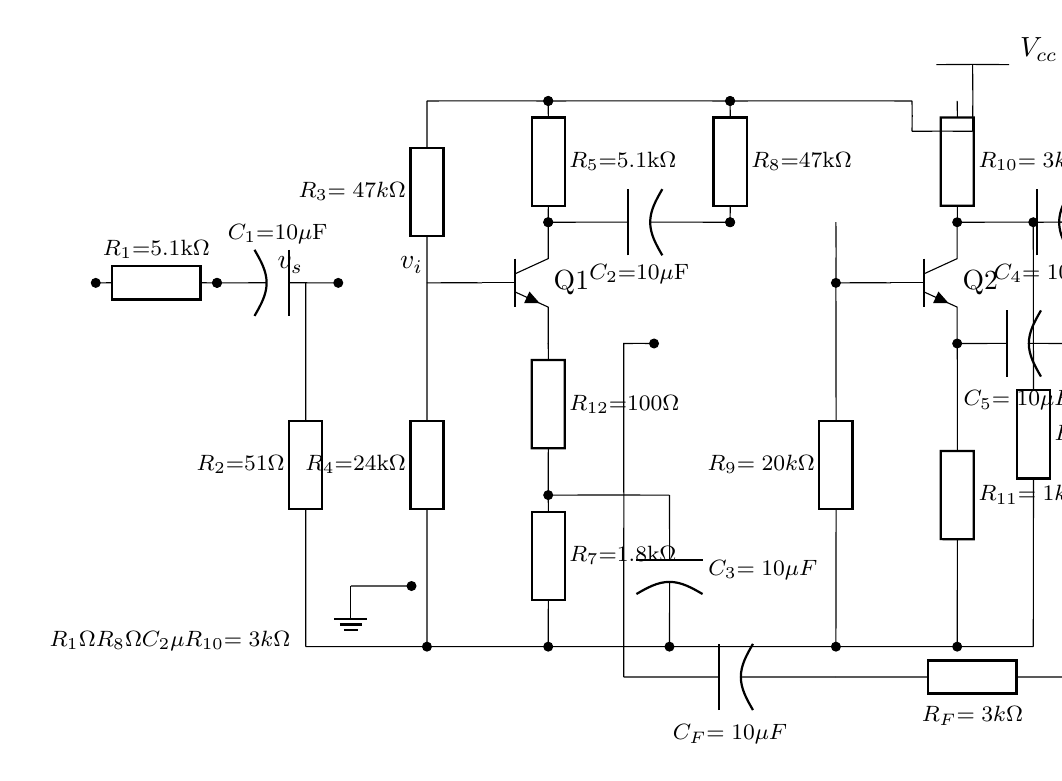
\begin{tikzpicture}[scale=1.54]
    \draw
(0,3) [R, l =\footnotesize $R_1\text{=5.1k}\Omega$, *-*] to (1,3)
(1,3) [pC, l=\footnotesize $C_1{=}10\mu\text{F}$, *-*] to (2,3)
;
    \draw
(3,3) node[npn](Q1){Q1}
(2,3) to [short] (Q1.B)
(Q1.E) to [R, l^=\footnotesize $R_{12}{=}100\Omega$] (3,1.5) to [R, l^=\footnotesize $R_7{=}1.8\text{k}\Omega$, -*] (3,0)
(Q1.C) [short, -*] to (3,3.5) to [R, l_=\footnotesize $R_5{=}5.1\text{k}\Omega$] (3,4.5)
(3,4.5) [short, *-*] to (4.5,4.5)
(4.5,4.5) [R, l =\footnotesize $R_8\text{=47k}\Omega$] to (4.5,3.5)
(4.5,3.5) [pC, l =\footnotesize $C_2\text{=10}\mu$\text{F}] to (3,3.5)
(4,0) [pC, l_=\footnotesize $C_3{=10}\mu{F}$,*-] to (4,1.25)
;
    \draw
(4,1.25) [short,-*] to (3,1.25)
;
    \draw
(1,3) [R, l_=\footnotesize $R_2\text{=51}\Omega$] to (1,0)
;
    \draw
(1,0) [short] to (7,0)
(7,0) [R, l_=\footnotesize $R_L\text{=1.5k}\Omega$] to (7,3.5)
;
    \draw
(7,3.5) [short, *-*] to (7.5,3.5)
;
    \draw
(2,3) [R, l_=\footnotesize $R_4\text{=24k}\Omega$,-*] to (2,0)
;
    \draw
(2,3) [R, l^=\footnotesize $R_3{=47k}\Omega$] to (2,4.5)
;
    \draw
(2,4.5) [short] to (3,4.5)
;
    \draw
(4.5,4.5) [short] to (6,4.5)
(6,4.5) [short] to (6,4.25)
(6,4.25) [short] to (6.5,4.25)
(6.5,4.25) [short] to (6.5,4.8)
;
    \draw
(6.2,4.8) [short] to (6.8,4.8)
;
    \draw
(5.5,3) node[npn](Q2){Q2}
(4.5,3) to [short] (Q2.B)
(Q2.E) to [R, l^=\footnotesize $R_{11}{=1k}\Omega$,-*] (5.5,0)
(Q2.C) [R, l_=\footnotesize $R_{10}{=3k}\Omega$] to (5.5,4.5)
(7,3.5) [pC,l^=\footnotesize $C_4{=10}\mu{F}$,-*] to (5.5,3.5)
;
    \draw
(6.5,0) [short,*-] to (6.5,2.5)
(6.5,2.5) [pC, l=\footnotesize $C_5{=10}\mu{F}$,-*] to (5.5,2.5)
;
    \draw
(4.5,3.5) [short,-*] to (4.5,3)
(4.5,3) [R, l_=\footnotesize $R_9{=20k}\Omega$, -*] to (4.5,0)
;
    \draw
(7,3) [short,*-] to (6.75,3)
;
    \draw
(6.75,3) [short] to (6.75,-0.25) [R,l=\footnotesize $R_F{=3k}\Omega$] to (4.5,-0.25)
;
    \draw
(4.5,-0.25) [pC, l=\footnotesize $C_F{=10}\mu{F}$] to (2.75,-0.25)
;
	\draw
(2.75,-0.25) [short] to (2.75,2.5) [short,-*] to (3,2.5)
;
    \draw
(1,0.5) [short,*-] to (0.5,0.5)
(0.5,0.5) node[ground](GND){}

{[anchor = south] (0,3) node{$v_s$}}
{[anchor = south] (1,3) node{$v_i$}}
{[anchor = south] (7.5,3.5) node{$v_o$}}
{[anchor = north] (6.5,5.1) node{$V_{cc}$ +12V}}
;
\end{tikzpicture}
\caption{负反馈放大电路}\label{cd}
\end{figure}

\section{实验内容}
凡是通过一定方式把放大电路的输出回路中某一个电量(电压或电流)的一部分或全部送回到输入回路中,这种电压或电流的反送过程叫做反馈。如果反馈到输入回路中的电量,具有加强输入信号的作用,是正反馈,反之是负反馈。判别正、负反馈的一个重要方法是“瞬时极性法”。\\
负反馈在电子线路中有着非常广泛的应用。虽然它使放大器的放大倍数降低,但能在多方面改善放大器的动态指标,如稳定放大器的放大倍数、改变放大器的输入输出电阻、减小非线性失真、扩展频带等等。因此,几乎所有的实用放大器都引入负反馈。\\
负反馈共有四种类型,即电压串联负反馈、电压并联负反馈、电流串联负反馈、电流并联负反馈。本实验电路是电压放大器。通常,电压放大器希望电压放大倍数尽可能稳定,输入电阻大,输出电阻小,所以,本实验电路引入的是电压串联负反馈。实验电路如图(\ref{cd})。
\begin{enumerate}
\item 测量开环放大器的静态参数\\
将图(\ref{cd})中的CF和RF支路开路。用数字万用表测量电路的静态参数,填写表(\ref{Q})。\\
对于本实验电路,由于$\beta$值较小,$I_{B1}$较大,$I_{B1}$在$R_3$上的电压降不能忽略,所以,在估算电路静态参数时必须计及$I_{B1}$,否则将出错。现在用计及IB1的方法估算第一级放大器的静态参数。
分别对$R_3$、$R_4$支路和$R_{12}$、$R_7$支路列电压方程,
\begin{eqnarray}
R_3(I_{B1}+I_{R4})+R_4I_{R4} &=& V_{cc}\\
R_4I_{R4}-V_{BE} &=& (\beta+1)I_{B1}(R_{12}+R_7)
\end{eqnarray}
解方程组可得:
\begin{eqnarray}
I_{B1} &=& \cfrac{R_4V_{cc}-(R_3+R_4)V_{BE}}{R_3R_4+(R_3+R_4)(R_{12}+R_7)(\beta+1)}\\\label{IB1}
I_{R4} &=& \cfrac{R_3V_{BE}+(R_{12}+R_7)(\beta+1)V_{cc}}{R_3R_4+(R_3+R_4)(R_{12}+R_7)(\beta+1)}\label{IR4}
\end{eqnarray}

若设$V_{BE}=$0.7V,$\beta$=30,则将他们代入式(\ref{IB1})得$I_{B1}\approx 41.74\mu V$,由此可得:\\
$I_{C1} = \beta I_{B1}\approx$1.252mA,$V_{C1} = V_{cc} - I_{C1}R_5\approx$5.61V,$V_{E1} = (\beta+1)I_{B1}(R_{12}+R_7)\approx$2.46V,$V_{CE1} = V_{C1} - V_{E1}\approx$3.15V\\
可见,第一级放大器的$Q_1$处于放大状态,电路静态点为$Q_1$(3.15V ,1.25mA),处于良好的放大状态。\\
若忽略$I_{B1}$在$R_3$上的压降,通常按如下方法做静态估算:\\
\begin{eqnarray}
V_{B1} &=& \cfrac{R_4}{R_3+R_4}V_{cc} \approx3.84V\\
V_{E1} &=& V_{B1} - V_{BE1} =3.84-0.7 = 3.14(V)\\
I_{C1} &\approx& I_{E1} = \cfrac{V_{E1}}{R_{12}+R_7}\approx1.65mA\\
V_{C1} &=& V_{cc} - R_5I_{C1}\approx3.57V
\end{eqnarray}
$Q_1$处于饱和状态,第一级放大电路不能正常工作。\\
对于本实验电路,计及基极电流的静态估算法是正确的。通过实验可以验证。
\item 开环放大器动态性能测量
\begin{enumerate}
\item 开环交流电压放大倍数测量
调整信号源,使$V_i$=1mV、f=10kHz。用交流毫伏表测量计算电路的交流电压放大倍数,填写表(\ref{AvAC})。
\item 取V$V_i$=1mV,改变频率,测量绘制整个开环放大器的幅频特性。方法和要求同实验1。找出整个放大器的下限频率和上限频率,填写表(\ref{fHL})。
\item 按实验1中给出的定义和表2.4的要求,测量整个放大电路的非线性谐波失真,填写表(\ref{harmonic})。
\begin{table}[!h]
\centering
\caption{测量谐波失真}
\label{harmonic}
\begin{tabular}{|c|c|c|c|c|c|c|c|}
\hline
                    & $V_i$(mV) & $d_{o2}$ & $d_{i2}$ & $d_2$ & $d_{o3}$ & $d_{i3}$ & $d_3$ \\ \hline
\multirow{2}{*}{开环} & 1         &          &          &       &          &         &       \\ \cline{2-8} 
                    & 10        &          &          &       &          &         &       \\ \hline
\multirow{2}{*}{闭环} & 1         &          &          &       &          &         &       \\ \cline{2-8} 
                    & 10        &          &          &       &          &         &       \\ \hline
\end{tabular}
\end{table}
\item 按实验1中给出的定义和表(\ref{rio})的要求,测量开环放大电路的输入、输出电阻,填写表(\ref{rio})。\\
开环输入电阻可用下列方法估算。开环时,输入电阻就是第一级放大器的输入电阻。设$\beta$=30,由计及$I_{B1}$静态分析法得到的$I_{B1}$开始:
\begin{eqnarray}
I_{E1} &=& (\beta+1)I_{B1}\approx 31\times 41.74\mu A\approx 1.294 mA\\
r_{be} &=& r_{bb'}+(\beta+1)\frac{26}{I_{E1}} = r_{bb'}+\frac{26}{I_{B1}} \approx 200+\frac{26}{0.04174}\approx 823\Omega\\
r_{iAC} &=& r_{be}+(\beta+1)R_{12} \approx 823+31\times 100 = 3923(\Omega)\\\label{2-6}
R_b &=& R_3||R_4 = 16.32\text{k}\Omega\\
r_{io} &=& R_b||r_{iAC} = \cfrac{16.32\times 3.923}{16.32+3.923} \approx 3.16\text{k}\Omega
\end{eqnarray}
其中,$r_{iAC}$为第一级放大器交流小信号等效输入电阻;$r_{io}$为开环输入电阻。
\end{enumerate}
\item 闭环放大器静态和动态性能测量\\
以下测量,若不作特别要求,输出端不接负载。
\begin{enumerate}
\item CF和RF支路如图(\ref{cd})连接。用数字万用表测量电路的静态参数,填写表(\ref{Q})。
由于本实验电路为交流负反馈,所以开环静态参数与闭环静态参数应该是一样的。
\item 调整信号源,使$V_i$=1mV、f=10kHz。用交流毫伏表测量计算电路的交流电压放大倍数,填写表(\ref{AvAC})。验证闭环放大倍数为
\begin{equation}
A_{VF} = \cfrac{A_V}{1+A_VF_V}
\end{equation}
其中$A_V$为开环放大倍数;$A_{VF}$为闭环放大倍数;$F_V = \frac{R_{12}}{R_F+R_{12}}$为电压反馈系数。只有当开环放大倍数与反馈系数的积$A_VF_V>>$1时,闭环放大倍数才能近似等于反馈系数的倒数。\\
电压串联负反馈减小了电压放大倍数,但提高了电压放大倍数的稳定性。在不考虑相位关系时,有
\begin{equation}
\cfrac{dA_{VF}}{A_{VF}} = \cfrac{1}{1+A_VF_V}\cfrac{dA_V}{A_V}
\end{equation}
表明引入电压串联负反馈后,电压放大倍数的相对变化是未加负反馈前的电压放大倍数的相对变化的1/(1+$A_VF_V$)倍,即闭环增益的稳定性提高了(1+$A_VF_V$)倍。
\item 取$V_i$=10mV,改变频率,测量绘制闭环放大器的幅频特性。方法和要求同实验1。找出整个放大器的下限频率和上限频率,填写表(\ref{fHL})。\\
负反馈扩展了放大器的通频带。引入负反馈后,放大器的上限频率$f_{HF}$和下限频率$f_{LF}$分别为:\\
$f_{HF} = (1+A_VF_V)f_H$,\\
$f_{LF} = f_L/(1+A_VF_V)$,\\
$f_{HF}$向高端扩展了$(1+A_VF_V)$倍, 向低端扩展了1/$(1+A_VF_V)$倍,使通频带加宽。
\item 按实验1中给出的定义和表(\ref{harmonic})的要求,测量闭环放大电路的非线性谐波失真,填写表(\ref{harmonic})。
\item 按实验1中给出的定义和表(\ref{rio})的要求,测量闭环放大电路的输入、输出电阻,填写表(\ref{rio})。\\
并联负反馈能降低输入电阻,串联负反馈则提高输入电阻。电压负反馈降低了输出电阻,使放大器趋向恒压源;电流负反馈提高了输出电阻,使放大器的输出端趋向恒流源。图(\ref{cd})引入的是电压串联负反馈,对整个放大器而言,使输入电阻提高,输出电阻降低,变化程度与反馈深度$(1+A_VF_V)$有关。\\
闭环输入阻抗可用下列方法估算。电压反馈网络的输出电阻为
\begin{equation}
r_{ofe} = R_F||R_{12} = 3000||100 \approx 96.7\Omega
\end{equation}
设开环放大倍数为360,在通带内,假设$A_V$的相移为零。引入电压串联负反馈后,闭环交流小信号等效输入电阻为
\begin{equation}
r_{ifAC} = r_{iAC}|1+A_VF_V|+r_{ofe}
 \approx 3923\times (1+360\times\frac{1}{30})+96.7
  \approx 51.096(\text{k}\Omega)
\end{equation}
其中,$r_{iAC}$为式(\ref{2-6})所示的第一级放大器交流小信号等效输入电阻,即开环交流小信号等效输入电阻。闭环输入电阻为
\begin{equation}
r_{if} = R_b||r_{ifAC} = 16.32||51.096 \approx 12.4\text{k}\Omega
\end{equation}
详细的推导可参考教材$^{\cite{jiaocai}}$。闭环后,放大器的输出阻抗的估算公式为
\begin{equation}
r_{of} = \cfrac{r_o}{|1+A_VF_V|}
\end{equation}
其中$r_o \approx R_{10}||R_L$。
\end{enumerate}
\end{enumerate}

\section{实验数据}
以下操作,如无特殊说明,均为有载情况。
\begin{enumerate}
\item 调整静态\\
开环和闭环状态下的负反馈放大器的静态工作点数据如表(\ref{Q}):\\
\begin{table}[!h]
\centering
\caption{测量静态参数}
\label{Q}
\begin{tabular}{|c|c|c|c|c|c|c|}
\hline
   & \multicolumn{3}{c|}{第一级}                & \multicolumn{3}{c|}{第二级}                \\ \hline
   & $V_{B1}$(V) & $V_{C1}$(V) & $V_{E1}$(V) & $V_{B2}$(V) & $V_{C2}$(V) & $V_{E2}$(V) \\ \hline
开环 & 2.863 & 6.001 & 2.231 & 2.631 & 6.000 & 1.985 \\ \hline
闭环 & 2.864 & 6.000 & 2.230 & 2.631 & 6.001 & 1.985 \\ \hline
\end{tabular}
\end{table}

其中,开环时调节好的滑动变阻器阻值分别为:\\
$R_{p1} = 25.678\text{k}\Omega$,$R_{p2} = 20.996\text{k}\Omega$\\
而固定电阻$R_3 = R_8 = 47\text{k}\Omega$。\\
显然,开环和闭环对放大器的静态工作点几乎没有影响,因为负反馈是交流特性,只在交流电路里体现。
\item 交流放大倍数\\
在$V_s = 104$mV下。测量放大器的交流放大倍数如表(\ref{AvAC}):
\begin{table}[H]
\centering
\caption{测量交流电压放大倍数}
\label{AvAC}
\begin{tabular}{|c|c|c|c|c|c|c|}
\hline
   & \multicolumn{3}{c|}{\multirow{2}{*}{输入输出电压(mV)}} & \multicolumn{3}{c|}{电压放大倍数} \\ \cline{1-1} \cline{5-7} 
   & \multicolumn{3}{c|}{}                            & 第一级      & 第二级      & 全电路   \\ \hline
   & $V_i$(mV)     & $V_{C1}$(mV)     & $V_o$(mV)     & $A_{V1}$ & $A_{V2}$ & $A_V$ \\ \hline
开环 & 1.004 & 18.463 & 1.086 & 18.389 & 58.82 & 1081.67 \\ \hline
闭环 & 1.007 & 0.555 & 29.960 & 0.551 & 53.982 & 29.752 \\ \hline
\end{tabular}
\end{table}
验证闭环放大倍数与开环放大倍数的关系:
\begin{eqnarray}
F_V &=& \cfrac{R_{12}}{R_F+R_{12}} = \cfrac{0.1\text{k}\Omega}{0.1\text{k}\Omega+3\text{k}\Omega} = \frac{1}{31}\\
A_{V} &=& 1081.67\\
A_{VF} &=& 29.752\\
\cfrac{A_V}{1+A_VF_V} &=& \cfrac{1081.67}{1+1081.67\times\frac{1}{31}} \approx 30.136 \approx A_{VF}
\end{eqnarray}
\item 幅频特性(通频带)\\
取中频10kHz,开环时,$V_{o} = 1.106$V,闭环时$V_o = 30.2$mV。测得数据如表(\ref{fHL}):
\begin{table}[!h]
\centering
\caption{测量幅频特性}
\label{fHL}
\begin{tabular}{|c|c|c|}
\hline
   & 下限频率$f_L$ & 上限频率$f_H$ \\ \hline
开环 & 754Hz & 240kHz \\ \hline
闭环 & 191Hz & 13.6MHz \\ \hline
\end{tabular}
\end{table}

验证负反馈放大电路对幅频特性的影响:\\
闭环后,放大电路的通频带得到了拓宽,闭环理论值应为开环时的$(1+A_VF_V)$或$\frac{1}{(1+A_VF_V)}$倍:
\begin{eqnarray}
f_{L\text{,闭环}} &=& \cfrac{f_L}{1+A_VF_V} \approx \cfrac{754}{35.9} \approx 21\text{Hz}\\
f_{H\text{,闭环}} &=& f_H\times (1+A_VF_V) \approx 240\times 35.9 \approx 8.6\text{MHz}
\end{eqnarray}
尽管具体数值与测量数据不是很相近,但是数量级大致正确,可以验证负反馈对幅频特性的影响。
\item 输入输出电阻\\
输入输出电阻的数据如表(\ref{rio}):
\begin{table}[!h]
\centering
\caption{测量输入输出电阻}
\label{rio}
\begin{tabular}{|c|c|c|c|c|c|c|c|c|}
\hline
   & \multicolumn{4}{c|}{测输入电阻$r_i$,$R_s$=5k$\Omega$}      & \multicolumn{4}{c|}{测输出电阻$r_o$}                  \\ \hline
   & \multicolumn{2}{c|}{测量值(mV)} & 测量计算值      & 理论估算值       & \multicolumn{2}{c|}{$V_o$(V)测量值} & 测量计算值 & 理论估算值 \\ \hline
   & $V_s$         & $V_i$        & $r_i$      & $r_i$     & 无负载       & 负载1.5k$\Omega$       & $r_o$ & $r_o$ \\ \hline
开环 & 100mV & 68.777mV & 11.234k$\Omega$ & 10.06k$\Omega$ & 0.323V & 111.822mV & 2.833k$\Omega$ & 3k$\Omega$ \\ \hline
闭环 & 100mV & 74.868mV & 15.193k$\Omega$ & 17.65k$\Omega$ & 3.086mV & 3.037mV & 24.2$\Omega$ & 27.86$\Omega$ \\ \hline
\end{tabular}
\end{table}

\textbf{测量值:}我们使用实验1中的相关公式计算输入输出电阻的测量值:
\begin{eqnarray}
r_i &=& \cfrac{R_s}{\frac{V_s}{V_i}-1}\\
r_o &=& \left(\frac{V_{\text{空载}}}{V_{\text{有载}}}-1\right)R_L
\end{eqnarray}
\textbf{理论值:}根据前文关于输入输出电阻的内容可以计算理论值:
\begin{enumerate}
\item 开环输入电阻\\
开环时,负反馈放大器的输入电阻就是第一级放大器的输入电阻。我们先使用实验1中的方法计算$\beta$值
\begin{eqnarray}
I_{c1} &=& \frac{V_{cc}-V_c}{R_5} = \frac{12V-6.001V}{5.1\text{k}\Omega} = 1.176\text{mA}\\
I_{b1} &=& \frac{V_{cc}-V_{b1}}{R_3+R_{p1}}-\frac{V_{b1}}{R_4} = \frac{12V-2.863V}{47\text{k}\Omega+25.678\text{k}\Omega} - \frac{2.863V}{24\text{k}\Omega} = 6.427\mu\text{A}\\
\beta &=& \frac{I_{c1}}{I_{b1}} \approx 182.971
\end{eqnarray}
再算出理论放大倍数:
\begin{eqnarray}
I_{e1} &=& (\beta+1)I_{b1} \approx 1.182\text{mA}\\
r_{be} &=& r_{bb'} + (\beta+1)\frac{26mV}{I_{e1}} \approx 4.362\text{k}\Omega\\
r_{iAC} &=& r_{be} + (\beta+1)R_{12} = 22.76\text{k}\Omega\\
R_{b1} &=& (R_3+R_{p1})||R_4 \approx 18.04\text{k}\Omega\\
r_{io} &=& R_{b1}||r_{iAC} \approx 10.06\text{k}\Omega
\end{eqnarray}
误差为:
\begin{equation}
Error(r_{i\text{,开环}}) = \cfrac{11.234-10.06}{10.06}\times 100\% \approx 11.67\%
\end{equation}
\item 闭环输入电阻\\
闭环时,输入电阻计算过程如下:
\begin{eqnarray}
r_{ofe} &=& R_F||R_{12} \approx 96.77\Omega\\
r_{ifAC} &=& r_{iAC}|1+A_VF_V|+r_{ofe} \approx 817.01\text{k}\Omega\\
r_{if} &=& R_{b1}||r_{ifAC} \approx 17.65\text{k}\Omega\\
\end{eqnarray}
误差为:
\begin{equation}
Error(r_{i\text{,闭环}}) = \cfrac{15.193-17.65}{17.65}\times 100\% \approx -13.92\%
\end{equation}
\item 开环输出电阻\\
开环时的输出电阻即为第二级放大电路的输出电阻,根据实验1的内容,可得:
\begin{equation}
R_o = R_{10} = 3\text{k}\Omega
\end{equation}
误差为:
\begin{equation}
Error(r_{o\text{,开环}}) = \cfrac{2.833-3}{3}\times 100\% \approx -5.567\%
\end{equation}
\item 闭环输出电阻\\
\begin{eqnarray}
r_{o} &\approx& R_{10}||R_L = \cfrac{3\text{k}\Omega\times 1.5\text{k}\Omega}{3\text{k}\Omega+1.5\text{k}\Omega} = 1\text{k}\Omega\\
r_{of} &=& \cfrac{r_o}{1+A_VF_V}\times \approx 27.86\Omega
\end{eqnarray}
误差为:
\begin{equation}
Error(r_{o\text{,闭环}}) = \cfrac{24.2-27.68}{27.68}\times 100\% \approx -13.14\%
\end{equation}
\end{enumerate}
\end{enumerate}

\section{误差分析}
\iffalse
\begin{enumerate}
\item 非深度负反馈\\
实验中反馈深度$A_VF_V \approx 34.9$,并不能算符合远远大于1这个条件,因此闭环放大倍数与理论值有误差。
\item 测量仪器示数\\
在测量闭环输出电阻时,测量仪器给出的空载和有载电压非常接近,而两者的比值除以1后作为分母,因此闭环输出电阻的值对这两个电压值十分敏感。它们的微小变化都可能引起闭环输出电阻的较大改变。而测量时仪器的示数一直不断跳动,给读数带来误差。
\end{enumerate}
\fi

\section{思考题}
\subsection{根据实验\text{1}和实验\text{2}的内容,小结负反馈闭环对放大电路性能的影响。}
\subsection{除实验内容以外,电压串联负反馈对放大器的性能还有哪些影响?}

%--------bib------------------
\bibliography{ref}
\end{document}